\documentclass[
  11pt,
  letterpaper,
   addpoints,
   answers
  ]{exam}

\usepackage{../exercise-preamble}

\begin{document}

\noindent
\begin{minipage}{0.47\textwidth}

\includegraphics[width=\textwidth]{../fcfm_die}
\end{minipage}
\begin{minipage}{0.53\textwidth}
\begin{center} 
\large\textbf{Electromagnetismo Aplicado} (EL3103-1) \\
\large\textbf{Clase auxiliar 3} \\
\normalsize Prof.~Benjamin Jacard H.\\
\normalsize Prof.~Aux.~Erik Saez A.
\end{center}
\end{minipage}

\vspace{0.5cm}
\noindent
\vspace{.85cm}

\begin{questions}
    %%%%%%%%%%%%%%%%%%%%%%%%%%%%
    \question Sean los siguientes problemas:
    \begin{enumerate}
        \item Encuentre una expresion para el potencial electrico dado el esquema de la figura.
    \end{enumerate}
    \begin{center}
        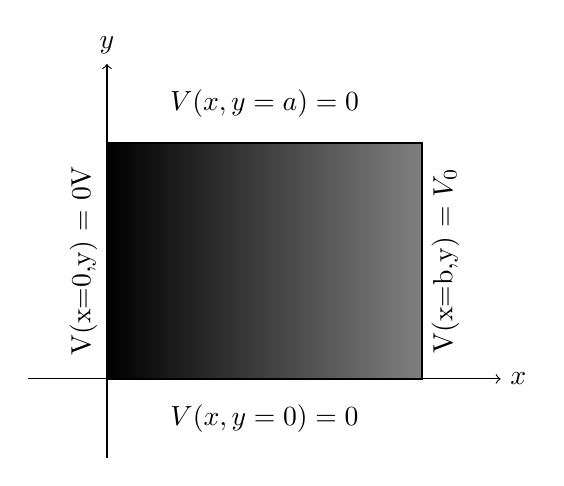
\begin{tikzpicture}
            % Dibuja el rectángulo con degradado
            \shade[left color=black, right color=gray] (0,0) rectangle (4,3);
        
            % Etiquetas de los ejes
            \draw[->] (-1,0) -- (5,0) node[right] {$x$};
            \draw[->] (0,-1) -- (0,4) node[above] {$y$};
        
            % Etiquetas de los potenciales
            \node at (2,-0.5) {$V(x,y=0) = 0$};
            \node at (2,3.5) {$V(x,y=a) = 0$};
            \node at (-0.3,1.5){\rotatebox{90}{V(x=0,y) = 0V}};
            \node at (4.3,1.5){\rotatebox{90}{V(x=b,y) = $V_{0}$}};
    
            % Contorno del rectángulo
            \draw[thick] (0,0) rectangle (4,3);
        \end{tikzpicture}
\end{center}
    %%%%%%%%%%%%%%%%%%%%%%%%%%%%
    \begin{solution}
        La resolucion viene dada por:
        \begin{enumerate}
            \item Se busca obtener una expresion para el potencial electrico en en todo el espacio dentro de este, para esto se utiliza la ecuacion de Laplace en coordenadas cartesianas, dado que no existe densidad de carga libre en el medio. Por tanto se tiene que:
            \begin{equation}
                \nabla^{2} V(x,y) = 0
            \end{equation}
            Luego reemplazando tenemos que:
            \begin{equation}
                \frac{\partial^{2}V}{\partial x^{2}} + \frac{\partial^{2}V}{\partial y^{2}} = 0
            \end{equation}
            Es posible asumir que las componentes no dependen entre si, por lo que se puede asumir una separacion de variables tal que:
            \begin{equation}
                V(x,y) = X(x)Y(y)
            \end{equation}
            Reemplazando sobre el Laplaciano tenemos que:
            \begin{align}
                \frac{\partial^{2}V}{\partial x^{2}} + \frac{\partial^{2}V}{\partial y^{2}} = 0\\
                Y\frac{\partial^{2}X(x)}{\partial x^{2}} + X\frac{\partial^{2}Y(y)}{\partial y^{2}} = 0\\
                Y\frac{\partial^{2}X(x)}{\partial x^{2}}= - X\frac{\partial^{2}Y(y)}{\partial y^{2}}\\
            \end{align}
            Luego tenemos una igualdad entre una funcion de $x$ y una funcion de $y$ que debe cumplirse para todo x e y, por lo que lla unica posibilidad sera la funcion constante tal que:
            \begin{align}
                \frac{1}{X(x)}\frac{\partial^{2}X(x)}{\partial x^{2}} &= -\frac{1}{Y(y)}\frac{\partial^{2}Y(y)}{\partial y^{2}} = k^{2}
            \end{align}
            Donde se asumira que la constante es positiva, por lo que se tendra que separando cada ecuacion:
            \begin{align}
                \frac{\partial^{2}X(x)}{\partial x^{2}} - k^{2}X(x) &= 0\\
                \frac{\partial^{2}Y(y)}{\partial y^{2}} + k^{2}Y(y) &= 0
            \end{align}
            Con lo que se tienen dos ecuaciones diferenciales ordinarias de segundo orden, las cuales se pueden resolver de manera independiente. Para la primera ecuacion se tiene que:
            \begin{align}
                \frac{\partial^{2}X(x)}{\partial x^{2}} - k^{2}X(x) &= 0\\
                X(x) &= Ae^{kx} + Be^{-kx}
            \end{align}
            luego para la segunda ecuacion se tiene que:
            \begin{align}
                \frac{\partial^{2}Y(y)}{\partial y^{2}} + k^{2}Y(y) &= 0\\
                Y(y) &= C\cos(ky) + D\sin(ky)
            \end{align}
            Luego tenemos que la expresion general para el potencial electrico es:
            \begin{align}
                V(x,y) &= X(x)Y(y)\\
                       &= \left(Ae^{kx} + Be^{-kx}\right)\left(C\cos(ky) + D\sin(ky)\right)
        \end{align}
        Luego debemos utilizar las condiciones de borde para determinar las constantes que caracterizan el sistema. Para la primera condicion de borde ($V(x,y=0)$) se tendra que:
        \begin{align}
            V(x,y=0) &= \left(Ae^{kx} + Be^{-kx}\right)\left(C\cos(0) + D\sin(0)\right) = 0\\
            &= \left(Ae^{kx} + Be^{-kx}\right)C = 0\\
        \end{align}
        Con lo que se obtiene que $C=0$, por lo que la ecuacion se reduce a:
        \begin{align}
            V(x,y) &= \left(Ae^{kx} + Be^{-kx}\right)\left(D\sin(ky)\right)\\
        \end{align}
        Luego para la segunda condicion de borde ($V(x=0,y)$) se tendra que:
        \begin{align}
            V(x=0,y) &= \left(Ae^{0} + Be^{0}\right)\left(D\sin(ky)\right) = 0\\
            &= (A+B)D\sin(ky) = 0
        \end{align}
        Esto se debe cumplir para cualquier valor de y, por lo que la unica opcion viene dada por $A = -B$ y por tanto se tiene que reemplazando sobre la ecuacion general
        \begin{align}
            V(x,y) &= \left(Ae^{kx} - Ae^{-kx}\right)\left(D\sin(ky)\right)\\
                   &= A\left(e^{kx} - e^{-kx}\right)D\sin(ky)
        \end{align}
        Luego utilizando la condicion de borde de $V(x,y=a)$ se tendra que:
        \begin{align}
            V(x,y=a) &= A\left(e^{kx} - e^{-kx}\right)D\sin(ka) = 0\\
            \Rightarrow& \sin(ka) = 0\\
            \Rightarrow& k = \frac{n\pi}{a} 
        \end{align}
        Luego reemplazando k en la expresion general se tendra que:
        \begin{align}
            V(x,y) &= A\left(e^{kx} - e^{-kx}\right)D\sin(ky)\\
                   &= A\left(e^{\frac{n\pi}{a}x} - e^{-\frac{n\pi}{a}x}\right)D\sin\left(\frac{n\pi}{a}y\right)
        \end{align}
        Luego podemos expresarlo en funcion del seno hiperbovico ($sinh(x)= \frac{e^{x}-e^{-x}}{2}$) y decimos que $C= 2AD$, por lo que:
        \begin{align}
            V(x,y) &= C\left(sinh\left(\frac{n\pi}{a}x\right)\right)\sin\left(\frac{n\pi}{a}y\right)
        \end{align}
        Se observa que este es funcion de n, ds decir que tendremos un numero infinito de soluciones y dado que el laplaciano es un operador lineal luego es posible realizar una superposicion de las soluciones, por lo que la solucion general sera: (\textit{Recordemos que por el teorema de unicidad el potencial es unico, no es que existan multiples soluciones}):
        \begin{align}
            V(x,y) &= \sum_{n=1}^{\infty}C_{n}\cdot sinh\left(\frac{n\pi}{a}x\right)\sin\left(\frac{n\pi}{a}y\right)
        \end{align}
        Luego debemos utilizar la ultima condicion de borde para obtener los valores del coeficiente $C_{n}$, es decir:
        \begin{align}
            V(x=b,y) &= \sum_{n=1}^{\infty}C_{n} \cdot sinh\left(\frac{n\pi}{a}b\right)\sin\left(\frac{n\pi}{a}y\right) = V_{0}\\
        \end{align}
        Estamos en presencia de una serie de Fourier, ademas al eliminar una de las variables se tiene que la serie de Fourier es ortogonal, por lo que se puede obtener el coeficiente $C_{n}$ mediante el producto interno entre la funcion y la base ortonormal, es decir:
        \begin{align}
            A_{n} = C_{n}sinh\left(\frac{n\pi}{a}b\right)
        \end{align}
        De esta manera tenemos que la constante sera:
        \begin{align}
            A_{n} &= \frac{2}{a}\int_{0}^{a}V(y)\sin\left(\frac{n\pi}{a}y\right)dy\\
            &= \frac{2}{a}\int_{0}^{a}V_{0}\sin\left(\frac{n\pi}{a}y\right)dy
        \end{align}
        Luego integrando la expresion $A_{n}$ tenemos:
        \begin{align}
            A_{n} &= \frac{2}{a}\int_{0}^{a}V_{0}\sin\left(\frac{n\pi}{a}y\right)dy\\
            &= \frac{2V_{0}}{a}(1-cos(n\pi))
        \end{align}
        Donde notamos que tendremos dos situacion, particulares segun sea el valor de n par o impar, por lo que se puede expresar como:
        \begin{equation}
            C_{n} = \frac{2V_{0}}{a}(1 - \cos(n\pi)) = 
            \begin{cases}
            0, & \text{si } n \text{ es par}, \\
            \frac{4V_{0}}{n \pi}, & \text{si } n \text{ es impar}.
            \end{cases}
            \end{equation}
        De esta manera tenemos que considerando unicamente los terminos impares, se puede expresar la solucion como:
        \begin{align}
            A_{n} = \frac{4V_{0}}{n \pi}sinh\left(\frac{n\pi}{a}b\right)\\
            C_{n} = \frac{4V_{0}}{n \pi \cdot sinh\left(\frac{n\pi b}{a}\right)}
        \end{align}         
        Luego es posible encontrar la expresion general para el potencial la cual viene dada por:
        \begin{equation}
            V(x,y) = \sum_{n=impar}^{\infty}C_{n} \cdot sinh\left(\frac{n\pi}{a}x\right)\sin\left(\frac{n\pi}{a}y\right)\\
            = \sum_{n=1}^{\infty}\frac{4V_{0}}{n \pi \cdot sinh\left(\frac{n\pi b}{a}\right)} \cdot sinh\left(\frac{n\pi}{a}x\right)\sin\left(\frac{n\pi}{a}y\right)
        \end{equation}
        \end{enumerate}
        Con lo que obtenemos la expresion para el potencial electrico en dos dimensiones, dado el esquema de la figura.
    \end{solution}
    %%%%%%%%%%%%%%%%%%%%%%%%%%%%
    \question  El campo eléctrico \( E(r, \phi) \) dentro de una cuña bidimensional \( (0 \leq \phi \leq \beta, r \leq R) \) limitada por un conductor perfecto conectado a tierra (figura 2) proporciona una visión de la naturaleza de los campos eléctricos cerca de esquinas conductoras. El potencial no puede ser singular cuando \( r \rightarrow 0 \), entonces se simplifica a la siguiente expresión (\( \alpha \) constante mayor a 0)
    \begin{equation}
        V (r, \phi) = A + B\phi + \sum_{\alpha > 0} C_{\alpha} r^{\alpha} \sin(\alpha \phi)
    \end{equation}
    \begin{enumerate}
        \item Determine los coeficientes \( A, B \) y \( \alpha \) a partir de las condiciones de borde. Luego de determinar \( \alpha \) encuentre la forma integral de calcular los \( C_{\alpha} \) a partir de \( f(\phi) \). Las condiciones de borde siguen la forma:
        
        \begin{equation}
            \left\{
            \begin{array}{l}
            V (r, 0) = 0 \quad r \in [0, R] \\
            V (r, \beta) = 0 \quad r \in [0, R] \\
            V (R, \phi) = f(\phi) \quad \phi \in [0, \beta]
            \end{array}
            \right.
        \end{equation}
        \item Cuando \( r \rightarrow 0 \) el potencial se puede aproximar por:
        \begin{equation}
            V(r, \phi) \approx r^{n/\beta} \sin\left(\frac{n\pi}{\beta}\right)
        \end{equation}
        
    Para esta expresión encuentre el campo eléctrico asociado y comente cualitativamente como se comporta el campo cuando \( r \rightarrow 0 \) en los casos \( \beta < \pi \), \( \beta = \pi \) y \( \beta > \pi \). Indicación: Puede ser útil recordar la expresión del gradiente en coordenadas polares. 
    \begin{center}
        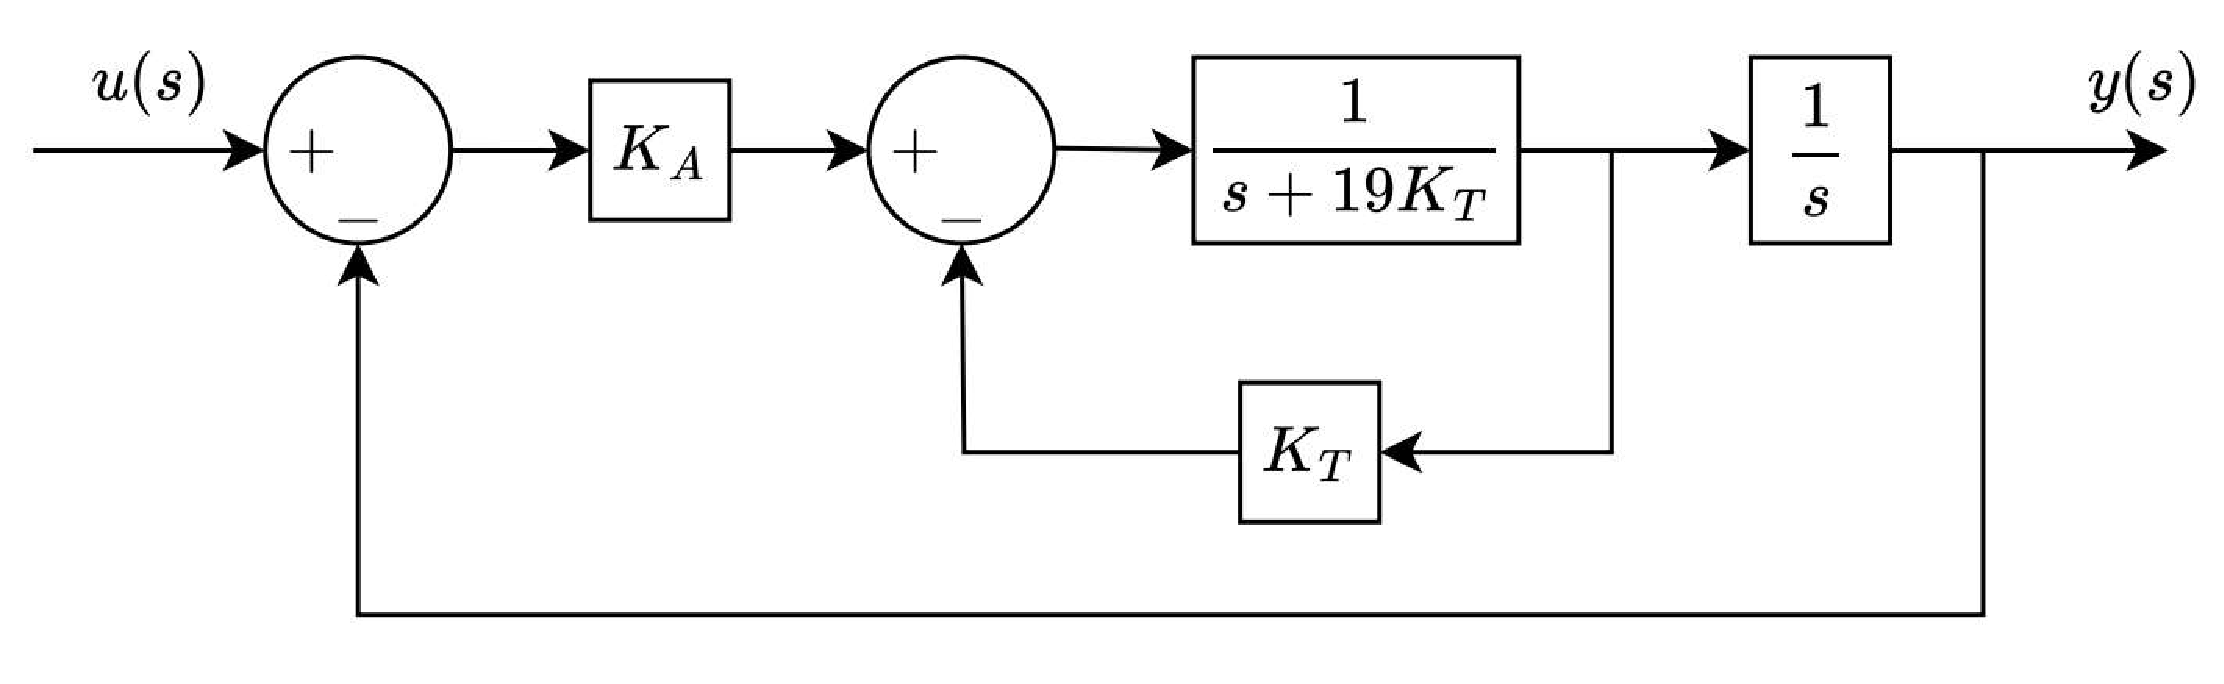
\includegraphics[width=0.6\textwidth]{Auxiliar_3_1}
        \captionof{figure}{Esquema general para los diferentes valores de $\beta$}
      \end{center}
    \end{enumerate}
    %%%%%%%%%%%%%%%%%%%%%%%%%%%%
    \begin{solution}
         La resolución viene dada por:
        \begin{enumerate}
            \item Dado que se busca obtener los diversos coeficiente A,B y $\alpha$, por lo que utilizando la primera condicion de borde se tiene que:
        \begin{align}
            V(r,0) &= A + B\cdot 0 + \sum_{\alpha > 0} C_{\alpha} r^{\alpha} \sin(\alpha \cdot 0) = 0 \\
                &\Rightarrow A = 0
        \end{align}
        Ademas dada esa condicion de borde sabemos que en todo el borde de la placa se tiene que cumplir que el potencial es cero (\textit{Recordemos que $r \in [0,R]$}), por lo tanto podemos evaluarlo en r=0 y se tiene que:
        \begin{align}
            V(r=0,\beta) &= B\cdot \phi + \sum_{\alpha > 0} C_{\alpha} 0^{\alpha} \sin(\alpha \cdot \phi) = 0 \\
                &= B\cdot \beta + 0 = 0\\
                &\Rightarrow B = 0
        \end{align}
        Por lo que se obtiene que A=B=0 y por tanto la ecuacion se reduce a:
        \begin{align}
            V(r,\phi) &= \sum_{\alpha > 0} C_{\alpha} r^{\alpha} \sin(\alpha \cdot \phi)\\
        \end{align}
        Dado que buscamos determinar el valor de $\alpha$, se debe utilizar la condicion de borde $V(R,\phi) = f(\phi)$, por lo que se tiene que:
        \begin{equation}
            V(r,\beta) = \sum_{\alpha > 0} C_{\alpha} r^{\alpha} \sin(\alpha \cdot \beta) = 0
        \end{equation}
        Para que tenga sentido la ecuacion (\textit{Si no feura el caso, deberia cumplirse que $C_{\alpha}=0  o R^{\alpha}$= 0 lo cual produce que el potencial siempre sea 0 y no es de interes}), la unica forma es que $sen(\alpha \cdot \phi) = 0$, por lo que se tiene que:
        \begin{align}
            \alpha \cdot \beta &= n\pi\\
            \Rightarrow \alpha &= \frac{n\pi}{\beta}
        \end{align}
        Luego reemplazando la expresion de $\alpha$ en la ecuacion del potencial se tiene que:
        \begin{align}
            V(r,\phi) &= \sum_{\alpha > 0} C_{\alpha} r^{\frac{n\pi}{\beta}} \sin\left(\frac{n\pi}{\beta} \cdot \phi\right)\\
            &= \sum_{n=1}^{\infty} C_{n} r^{\frac{n\pi}{\beta}} \sin\left(\frac{n\pi}{\beta} \cdot \phi\right)
        \end{align}
        Luego debemos determinar las constantes $C_{n}$, para lo cual se utiliza la condicion de borde $V(R,\phi) = f(\phi)$, por lo que se tiene que:
        \begin{align}
            V(R,\phi) &= \sum_{n=1}^{\infty} C_{n} R^{\frac{n\pi}{\beta}} \sin\left(\frac{n\pi}{\beta} \cdot \phi\right)= f(\phi)
        \end{align}
        Luego se tiene una serie de Fourier, por lo que se puede obtener el coeficiente $C_{n}$ mediante el producto interno entre la funcion y la base ortonormal, es decir:
        \begin{equation}
            A_{n} = C_{n} R^{\frac{n\pi}{\beta}}
        \end{equation}
        Con lo que tenemos que 
        \begin{align}
            C_{n} &= \frac{2}{\beta \cdot R^{\frac{n \pi }{\beta}}}\int_{0}^{\beta}f(\phi)\sin\left(\frac{n\pi}{\beta} \cdot \phi\right)d\phi
        \end{align}    
    Con lo que se obtiene la expresion para el potencial electrico en la cuña bidimensional, dado el esquema de la figura.
    \item tenemos que cuando el potencial ($r \rightarrow 0 $), en los casos $\beta < \pi$ , $\beta = \pi$ y $\beta > \pi$ se tiene que: 
    \begin{align}
        V(r,\phi) \approx r^{\frac{\pi}{\beta}}\sin\left(\frac{n\pi \phi}{\beta}\right)
    \end{align}
    Notamos que en este caso predomina m = 1, luego tenemos que el campo electrico asociado sera:
    \begin{align}
        E = -\nabla V 
    \end{align}
    Sabemos que el gradiente en coordenadas polares es:
    \begin{align}
        \nabla V &= \hat{r} \frac{\partial V}{\partial r} + \hat{\phi} \frac{1}{r}\frac{\partial V}{\partial \phi}
    \end{align}
    Con lo que se obtiene que:
    \begin{align}
        \mathbf{E} = -\nabla V = -\frac{\pi}{\beta} r^{\frac{\pi}{\beta}-1} \left[ \hat{r} \sin\left( \frac{\pi \phi}{\beta} \right) + \hat{\phi} \cos\left( \frac{\pi \phi}{\beta} \right) \right]
    \end{align}
    Una vez obtenido el campo electrico, se puede analizar el comportamiento del mismo en los diferentes casos:

    \begin{itemize}
        \item \textbf{Caso \(\beta < \pi\)}: En esta situación tenemos que \(E \rightarrow 0\) cuando \(r \rightarrow 0\).
        \item \textbf{Caso \(\beta = \pi\)}: En este caso el campo eléctrico se comporta como un vector constante dirigido verticalmente.
        \item \textbf{Caso \(\beta > \pi\)}: En este caso el campo eléctrico diverge, es decir, se tiene que \(E \rightarrow \infty\), por lo que el campo eléctrico diverge en la esquina (\(\beta \rightarrow 2\pi\)).
    \end{itemize}
    
    \end{enumerate}
    \end{solution}
    %%%%%%%%%%%%%%%%%%%%%%%%%%%
    \question  Una placa de un material con constante $\epsilon_{0}$ posee dimensiones de \(8 \, \text{cm} \times 8 \, \text{cm}\), y se le aplica potencial como muestra la figura.
    \begin{center}
        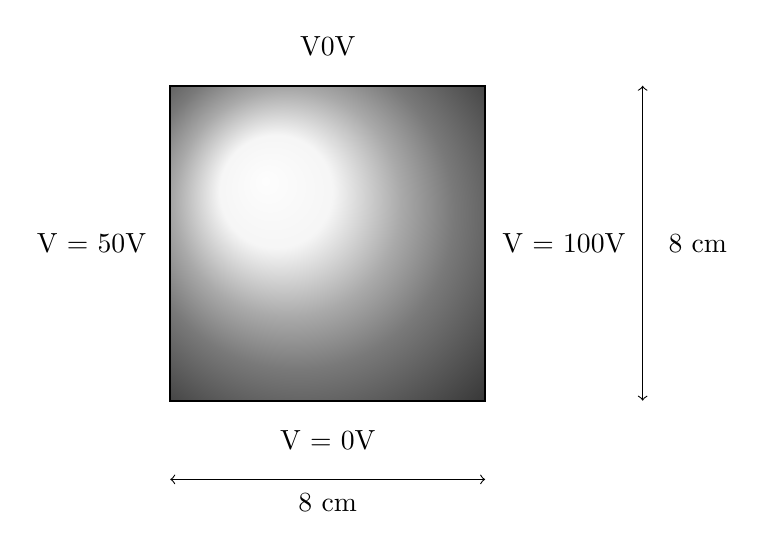
\begin{tikzpicture}
            % Degradado
            \fill[ball color=gray!10] (0,0) rectangle (4,4);
            
            % Dibujo de la placa
            \draw[thick] (0,0) rectangle (4,4); % rectángulo para la placa
            
            % Líneas de los bordes de la placa
            \node at (-1, 2) {V = 50V};
            \node at (5, 2) {V = 100V};
            \node at (2, -0.5) {V = 0V};
            \node at (2, 4.5) {V0V};
            
            % Etiquetas de las dimensiones
            \draw[<->] (0, -1) -- (4, -1); 
            \node at (2, -1.3) {8 cm}; 
            \draw[<->] (6, 0) -- (6, 4); 
            \node at (6.7, 2) {8 cm}; 
        \end{tikzpicture}
    \end{center}
    \begin{enumerate}
        \item Determine el potencial en el centro de la placa y el campo eléctrico en el centro de la placa.
        \item Suponga que alguna persona maldadosa decide insertar dos materiales con constantes $\epsilon_{1}$ y $\epsilon_{2}$, estos se dividen en el medio de la placa. En que cambia el sistema?
        \item No solo con esto, decide posteriormente eliminar los diferentes materiales e insertar una densidad de carga $\rho = 5 \epsilon_{0}$. En que se ve afectado el sistema? \textbf{Propuesto}
    \end{enumerate}
    %%%%%%%%%%%%%%%%%%%%%%%%%%%
    \begin{solution}
        \begin{enumerate}
            \item Para determinar el potencial en el centro de la placa, es necesario FDM (Finite Difference Method) o el método de diferencias finitas. Este consiste en discretizar el espacio de la siguiente manera:
            \begin{center}
                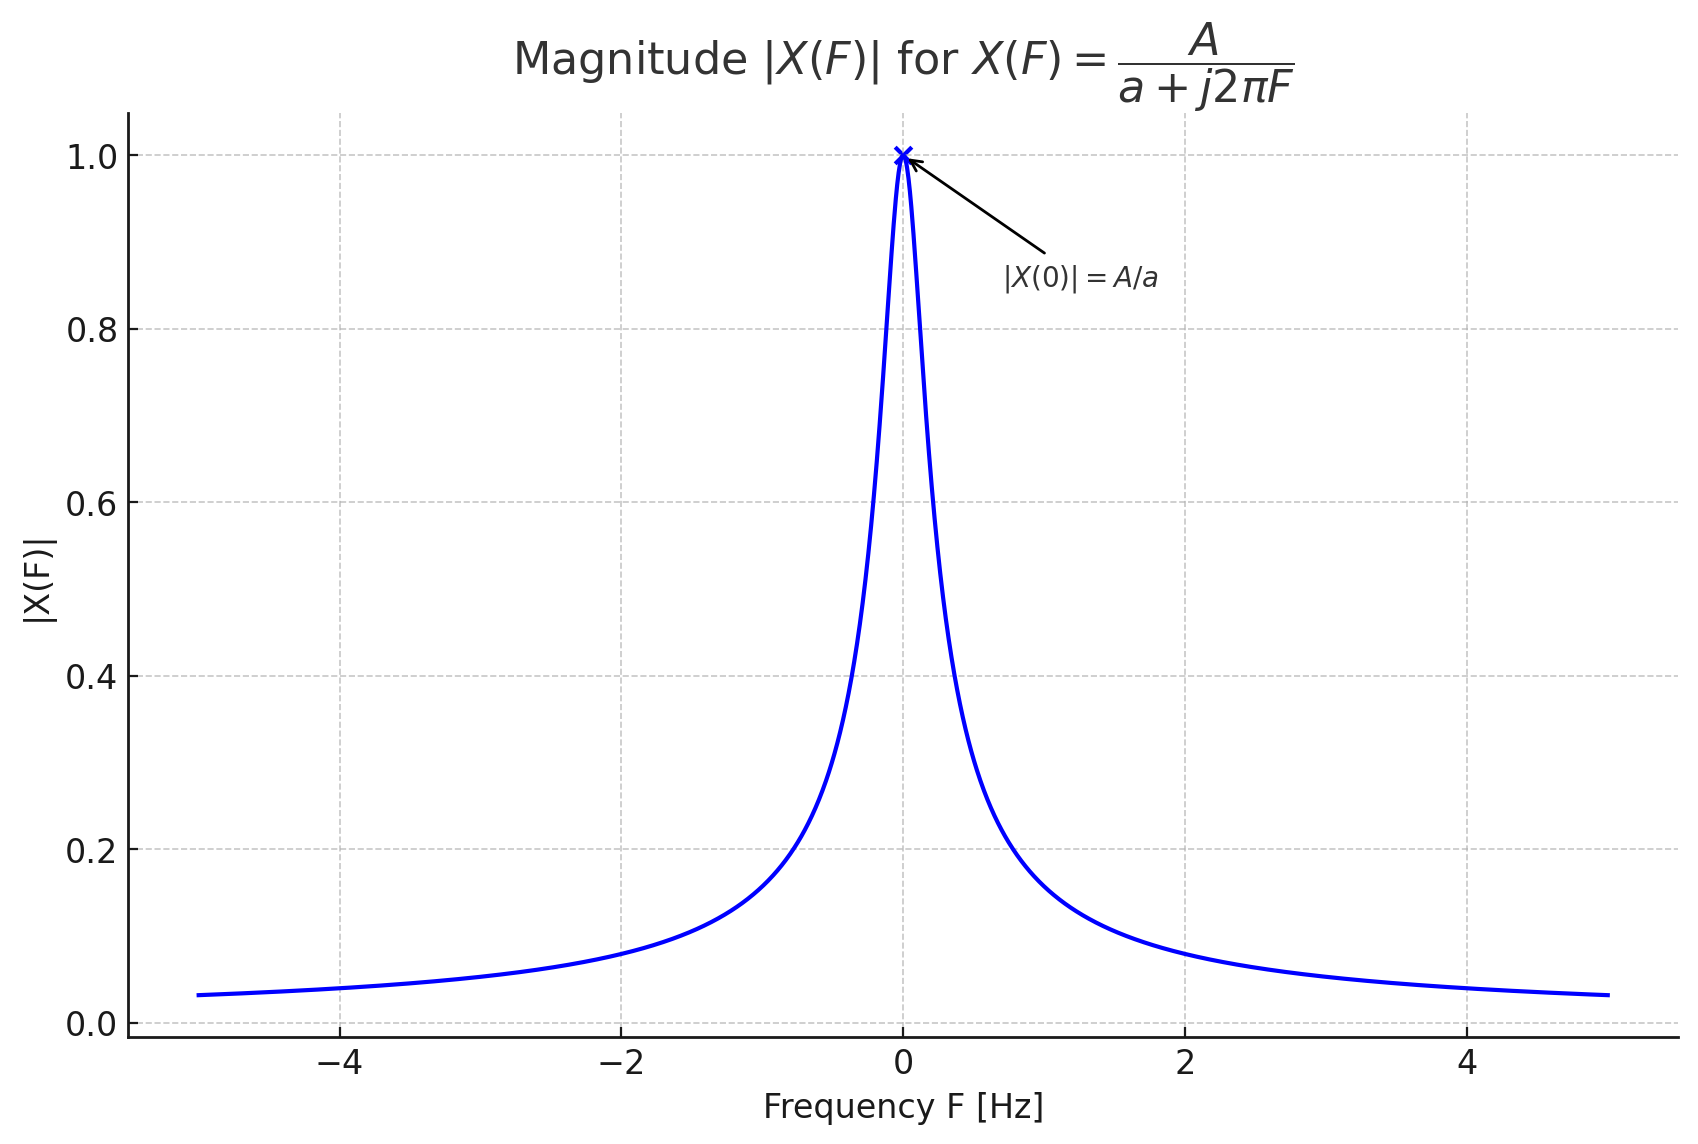
\includegraphics[width=0.5\textwidth]{Auxiliar_3_2}
                \captionof{figure}{Esquema general para los diferentes valores de $\beta$}
              \end{center}
            De tal manera que tenemos que asumiendo que el potencial depende de V(x,y):
            \begin{equation}
                V(i,j) = V(x_{i},y_{j})
            \end{equation}
            Luego asumiendo que la densidad de carga tambien varia punto a punto, se cumple que:
            \begin{align}
                \nabla^{2}V(x,y) = -\frac{\rho(x,y)}{\epsilon}
            \end{align}
            Reemplazando:
            \begin{align}
                \frac{\partial^{2}V(i,j)}{\partial x^{2}} + \frac{\partial^{2}V(i,j)}{\partial y^{2}} = -\frac{\rho(i,j)}{\epsilon}
            \end{align}
            Con lo ultimque podemos aproximar la derivada de la siguiente manera:
            \begin{align}
                \frac{\partial^{2}V(i,j)}{\partial x^{2}} &\approx \frac{V(i+1,j) - 2V(i,j) + V(i-1,j)}{(h)^{2}}\\
                \frac{\partial^{2}V(i,j)}{\partial y^{2}} &\approx \frac{V(i,j+1) - 2V(i,j) + V(i,j-1)}{(h)^{2}}
            \end{align}
            Por lo tanto tenemos que:
            \begin{align}
                \frac{V(i+1,j) - 2V(i,j) + V(i-1,j)}{(h)^{2}} + \frac{V(i,j+1) - 2V(i,j) + V(i,j-1)}{(h)^{2}} = -\frac{\rho(i,j)}{\epsilon}
            \end{align}
            Por lo tanto tenemos que el potencial $V(i,j)$ se puede expresar como:
            \begin{align}
                V(i,j) = \frac{1}{4} \left[ V(i-1,j) + V(i+1,j) + V(i,j-1) + V(i,j+1) + \frac{\rho(i,j)h^2}{\varepsilon} \right]
            \end{align}
            Lo que permite entender que para calcular el potencial en el punto(i,j) se necesitan los puntos alrededor formando lo que se conoce como estrella de 5 puntos.
            \begin{center}
                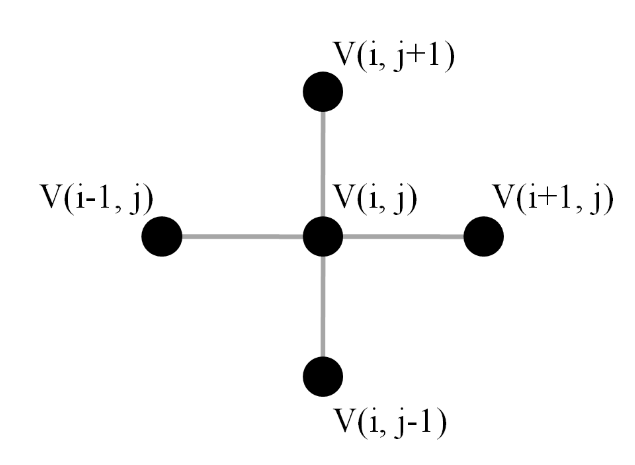
\includegraphics[width=0.3\textwidth]{Auxiliar_3_3}
                \captionof{figure}{Esquema general para los diferentes valores de $\beta$}
              \end{center}
            Para el primer apartado, se busca obtener el potencial en el centro de la placa, por lo que debemos dividir el espacio, en particular se toma h=2, tal que:
            \begin{center}
                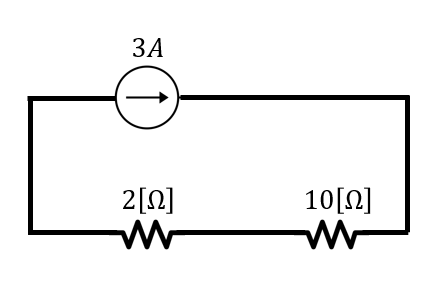
\includegraphics[width=0.3\textwidth]{Auxiliar_3_4}
                \captionof{figure}{Esquema general para los diferentes valores de $\beta$}
              \end{center}
            Por lo que las ecuaciones seran:
            \begin{align}
                V_1 &= \frac{1}{4} \left(50 + V_2 + V_4\right) \\
                V_2 &= \frac{1}{4} \left(V_1 + V_3 + V_5\right) \\
                V_3 &= \frac{1}{4} \left(V_2 + V + 6 + 100\right) \\
                V_4 &= \frac{1}{4} \left(V_1 + V_5 + V_7 + 50\right) \\
                V_5 &= \frac{1}{4} \left(V_2 + V_4 + V_6 + V_8\right) \\
                V_6 &= \frac{1}{4} \left(V_3 + V_5 + V_9 + 100\right) \\
                V_7 &= \frac{1}{4} \left(V_4 + V_8 + 50\right) \\
                V_8 &= \frac{1}{4} \left(V_5 + V_7 + V_9\right) \\
                V_9 &= \frac{1}{4} \left(V_6 + V_8 + 100\right)
                \end{align}
            Las cuales expresada en un sistema lineal de matrices:
            \begin{equation}
                \begin{bmatrix}
                -4 & 1 & 0 & 1 & 0 & 0 & 0 & 0 & 0 \\
                1 & -4 & 1 & 0 & 1 & 0 & 0 & 0 & 0 \\
                0 & 1 & -4 & 0 & 0 & 1 & 0 & 0 & 0 \\
                1 & 0 & 0 & -4 & 1 & 0 & 0 & 0 & 0 \\
                0 & 1 & 0 & 1 & -4 & 1 & 0 & 0 & 0 \\
                0 & 0 & 1 & 0 & 1 & -4 & 1 & 0 & 0 \\
                0 & 0 & 0 & 1 & 0 & 1 & -4 & 1 & 0 \\
                0 & 0 & 0 & 0 & 1 & 0 & 1 & -4 & 1 \\
                0 & 0 & 0 & 0 & 0 & 1 & 0 & 1 & -4
                \end{bmatrix}
                \begin{bmatrix}
                V_1 \\
                V_2 \\
                V_3 \\
                V_4 \\
                V_5 \\
                V_6 \\
                V_7 \\
                V_8 \\
                V_9
                \end{bmatrix}
                =
                \begin{bmatrix}
                -50 \\
                0 \\
                -100 \\
                -50 \\
                0 \\
                -100 \\
                -50 \\
                0 \\
                -100
                \end{bmatrix}
                \end{equation}
            Luego se debe resolver el sistema matricial que es de la forma:
            \begin{align}
                A \cdot V = B
            \end{align}      
            Al resolverlo entrega como valor para V(5,5)= 37.5 
            \item Para el segundo apartado, se tiene que al insertar los materiales, se debe considerar que la constante dielectrica cambia, por lo que el potencial en el centro de la placa sera diferente, por lo que se tendra el sigueinte esquema:
            \begin{center}
                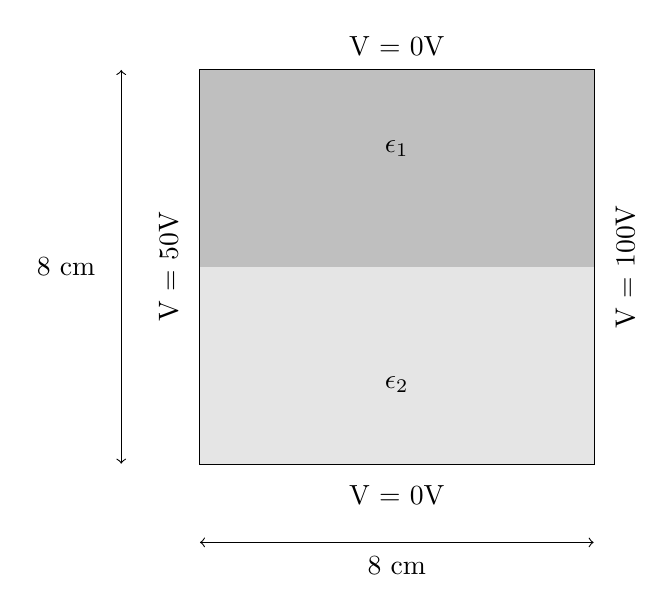
\begin{tikzpicture}[scale=1]  % Reducir el tamaño de la figura
    
        % Dibuja la placa
                \draw[thick] (0,0) rectangle (5,5); % rectángulo para la placa
        
        % Agregar degradado a las dos regiones
                \begin{scope}
                    \fill[gray!50] (0,2.5) rectangle (5,5); % Sombreado para \epsilon_1
                    \node at (2.5, 4) {$\epsilon_1$}; % Etiqueta para \epsilon_1
                \end{scope}
        
        \begin{scope}
            \fill[gray!20] (0,0) rectangle (5,2.5); % Sombreado para \epsilon_2
            \node at (2.5, 1) {$\epsilon_2$}; % Etiqueta para \epsilon_2
        \end{scope}

        % Líneas de los valores de V
        \node at (2.5, 5.3) {V = 0V};
        \node at (2.5, -0.4) {V = 0V};
        \node at (-0.4, 2.5) {\rotatebox{90}{V = 50V}};
        \node at (5.4, 2.5) {\rotatebox{90}{V = 100V}};

        % Etiquetas de las dimensiones
        \draw[<->] (0, -1) -- (5, -1); 
        \node at (2.5, -1.3) {8 cm}; 
        \draw[<->] (-1, 0) -- (-1, 5); 
        \node at (-1.7, 2.5) {8 cm}; 
    \end{tikzpicture}
\end{center}
        Por lo que al dividir el espacio se tendra que:
  
        \begin{center}
            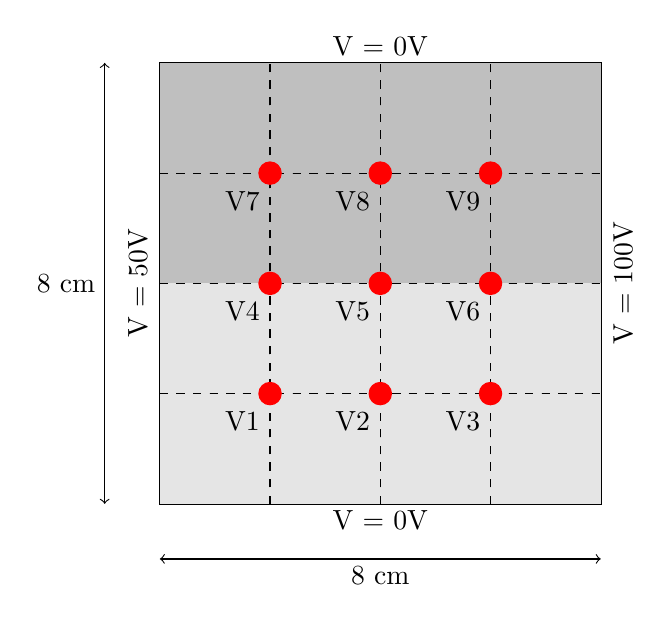
\begin{tikzpicture}[scale=0.7]  % Reducir el tamaño de la figura
            
                % Dibuja la placa
                \draw[thick] (0,0) rectangle (8,8); % rectángulo para la placa
                
                % Agregar degradado a las dos regiones
                \begin{scope}
                    \fill[gray!50] (0,4) rectangle (8,8); % Sombreado para \epsilon_1
                    \node at (4, 6) {$\epsilon_1$}; % Etiqueta para \epsilon_1
                \end{scope}
                
                \begin{scope}
                    \fill[gray!20] (0,0) rectangle (8,4); % Sombreado para \epsilon_2
                    \node at (4, 2) {$\epsilon_2$}; % Etiqueta para \epsilon_2
                \end{scope}
                
                % Líneas de los valores de V
                \node at (4, 8.3) {V = 0V};
                \node at (4, -0.3) {V = 0V};
                \node at (-0.4, 4) {\rotatebox{90}{V = 50V}};
                \node at (8.4, 4) {\rotatebox{90}{V = 100V}};
                
                % Dibuja la cuadrícula
                \foreach \i in {1, 2, 3} {
                    \foreach \j in {1, 2, 3} {
                        % Dibuja las líneas de la cuadrícula
                        \draw[dashed] (\i*2, 0) -- (\i*2, 8); % Líneas verticales
                        \draw[dashed] (0, \j*2) -- (8, \j*2); % Líneas horizontales
                    }
                }
                
                % Coloca los puntos rojos por encima de las líneas y las etiquetas de V
                \foreach \i in {1, 2, 3} {
                    \foreach \j in {1, 2, 3} {
                        % Coloca los puntos rojos encima de las líneas
                        \node[fill=red,circle,inner sep=3pt] at (\i*2, \j*2) {}; 
                    }
                }
        
                % Etiquetas de V en el orden correcto, de izquierda a derecha y de abajo a arriba
                \node at (1.5, 1.5) {V1};
                \node at (3.5, 1.5) {V2};
                \node at (5.5, 1.5) {V3};
                \node at (1.5, 3.5) {V4};
                \node at (3.5, 3.5) {V5};
                \node at (5.5, 3.5) {V6};
                \node at (1.5, 5.5) {V7};
                \node at (3.5, 5.5) {V8};
                \node at (5.5, 5.5) {V9};
                
                % Etiquetas de las dimensiones
                \draw[<->] (0, -1) -- (8, -1); 
                \node at (4, -1.3) {8 cm}; 
                \draw[<->] (-1, 0) -- (-1, 8); 
                \node at (-1.7, 4) {8 cm}; 
                
            \end{tikzpicture}
        \end{center}
        

        Luego usaremos nuevamente la expresion de la estrella de 5 puntos, dado por:
        \begin{align}
            V(i,j) = \frac{1}{4} \left[ V(i-1,j) + V(i+1,j) + V(i,j-1) + V(i,j+1) + \frac{\rho(i,j)h^2}{\varepsilon} \right]
        \end{align}
        Pero ahora debemos considerar el hecho de que los puntos ubicados entre los diferentes medios vendran dado por ejemplo para $V_{5} $ como:
        \begin{equation}
            V_{5} = \frac{1}{2(\epsilon_{1}+\epsilon_{2})} \left[ \frac{1}{2}(\epsilon_{1}+\epsilon_{2}) V_{4} +  \frac{1}{2}(\epsilon_{1}+\epsilon_{2}) V_{6} + \epsilon_{1}V_{8} + \epsilon_{2} V_{2} \right]
        \end{equation}
        Luego extendiendo esta idea tenemos que el set de ecuaciones vendra dado por:
        \begin{align}
            V_1 &= \frac{1}{4} \left( V_4 + V_2 + 50 \right) \\
            V_2 &= \frac{1}{4} \left( V_1 + V_5 + V_3 \right) \\
            V_3 &= \frac{1}{4} \left( V_2 + V_6 + 100 \right) \\
            V_4 &= \frac{1}{2(\epsilon_1 + \epsilon_2)} \left[ \epsilon_2 V_1 + \frac{1}{2} (\epsilon_1 + \epsilon_2) V_5 + \epsilon_1 V_7 + 50 \right] \\
            V_5 &= \frac{1}{2 (\epsilon_1 + \epsilon_2)} \left[ \epsilon_2 V_2 + \frac{1}{2} (\epsilon_1 + \epsilon_2) (V_4 + V_6) + \epsilon_1 V_8 \right] \\
            V_6 &= \frac{1}{2 (\epsilon_1 + \epsilon_2)} \left[ \epsilon_2 V_3 + \frac{1}{2} (\epsilon_1 + \epsilon_2) V_5 + \epsilon_1 V_9 + 100 \right] \\
            V_7 &= \frac{1}{4} \left( V_1 + V_8 + 50 \right) \\
            V_8 &= \frac{1}{4} \left( V_7 + V_5 + V_9 \right) \\
            V_9 &= \frac{1}{4} \left( V_8 + V_6 + 100 \right)
            \end{align}
            Luego en forma matricial tendremos que:
\[
\begin{bmatrix}
-4 & 1 & 0 & 0 & 0 & 0 & 0 & 0 & 0 \\
1 & -4 & 1 & 0 & 0 & 0 & 0 & 0 & 0 \\
0 & 1 & -4 & 0 & 0 & 0 & 0 & 0 & 0 \\
0 & 0 & 0 & -2(\epsilon_1 + \epsilon_2) & \epsilon_2 & 0 & \epsilon_1 & 0 & 0 \\
0 & 0 & 0 & \epsilon_2 & -2(\epsilon_1 + \epsilon_2) & \epsilon_2 & 0 & \epsilon_1 & 0 \\
0 & 0 & 0 & 0 & \epsilon_2 & -2(\epsilon_1 + \epsilon_2) & \epsilon_2 & 0 & \epsilon_1 \\
0 & 0 & 0 & 0 & 0 & \epsilon_2 & -4 & 0 & 0 \\
0 & 0 & 0 & 0 & 0 & 0 & \epsilon_2 & -4 & 0 \\
0 & 0 & 0 & 0 & 0 & 0 & 0 & \epsilon_2 & -4
\end{bmatrix}
\begin{bmatrix}
V_1 \\
V_2 \\
V_3 \\
V_4 \\
V_5 \\
V_6 \\
V_7 \\
V_8 \\
V_9
\end{bmatrix}
=
\begin{bmatrix}
-50 \\
0 \\
0 \\
-50 \\
0 \\
-50 \\
0 \\
-50 \\
-100
\end{bmatrix}
\]
\item \textbf{Propuesto}
    \end{enumerate}
\end{solution}
%%%%%%%%%%%%%%%%%%%%%%%%%%%
\end{questions}
\newpage
%%%%%%%%%%%%%%%%%%%%%%%%%%%

\end{document}